\section*{Comunicazioni analogiche}

Amplitude Modulation Dual Side Band (AM-DSB) is one of the simplest forms of modulation, generalmente utilizzata per trasmettere solo la voce. The signal \( s_{DSB}(t) \) is 

\begin{equation}
s_{DSB}(t) = A_c m(t) \cos(2\pi f_c t)
\end{equation}
where:
\begin{itemize}
  \item \( m(t) \) is the modulating signal or the message.
  \item \( A_c \) is the amplitude of the carrier signal.
  \item \( \cos(2\pi f_c t) \) is the carrier wave at frequency \( f_c \).
\end{itemize}

The frequency spectrum of AM-DSB shows two sidebands, each located at \( f_c \pm W \) ans \( -f_c \pm W \), where \( W \) is the bandwidth of the message signal. These sidebands carry the same information, hence the term 'dual sideband'.

Taking the Fourier transform of \( s_{DSB}(t) \), we obtain the frequency domain representation \( S_{DSB}(f) \):
\begin{equation}
S_{DSB}(f) = \frac{1}{2} A_c [M(f - f_c) + M(f + f_c)]
\end{equation}
where \( M(f) \) is the Fourier transform of \( m(t) \).
Sebbene la componente negativa possa essere trascurata adesso la traslazione del segnale alla frequenza $f_c >> $ comporta un'occupazione di banda di $2W$ per ogni lato, ma la ciò comporta uno spreco in quanto si ha duplicazione di informazione. 
\subsection*{Properties}
\begin{itemize}
  \item AM-DSB is a linear modulation technique since the modulated signal is a linear combination of \( m(t) \) and \( \cos(2\pi f_c t) \).
  \item Due to the modulation, the message signal is translated to higher frequencies, which can be efficiently transmitted over long distances.
  \item AM-DSB is power inefficient since the carrier contains no information but consumes power.
\end{itemize}



\subsection*{Applications}
AM-DSB is widely used in traditional AM radio broadcasting. Despite its simplicity, it is not the most power-efficient mode of transmission. In modern communications, variations like Single Sideband (SSB) or Suppressed Carrier (SC) are more frequently used to conserve bandwidth and power.
\begin{tikzpicture}
\begin{axis}[
    title={AM-DSB Modulation},
    xlabel={Time},
    ylabel={Amplitude},
    axis lines=middle,
    ymax=2,
    ymin=-2,
    xtick=\empty,
    ytick=\empty,
    clip=false,
    no markers,
    width=10cm,
    height=5cm
]
% Modulating signal m(t)
\addplot [domain=0:2*pi, samples=100, name path=m] {sin(deg(x))};
\addlegendentry{$m(t)$}

% Carrier signal Ac*cos(2*pi*f*t)
\addplot [domain=0:2*pi, samples=100, name path=carrier] {1.5*cos(deg(5*x))};
\addlegendentry{$A_c \cos(2\pi f_c t)$}

% Modulated signal Ac*m(t)*cos(2*pi*f*t)
\addplot [domain=0:2*pi, samples=100, red, name path=am] {1.5*sin(deg(x))*cos(deg(5*x))};
\addlegendentry{$s_{DSB}(t)$}

% Adding dashed lines for envelops
\addplot [domain=0:2*pi, samples=100, dashed, name path=upper] {1.5*sin(deg(x))};
\addplot [domain=0:2*pi, samples=100, dashed, name path=lower] {-1.5*sin(deg(x))};

% Filling the envelope
\addplot[fill=gray!30] fill between[of=upper and lower];

\end{axis}
\end{tikzpicture}

\begin{tikzpicture}[>=Stealth]
    % Blocks
    \node (m) at (0,0) {$m(t)$};
    \node[draw, right=2cm of m] (multiplier) {Multiplier};
    \node[draw, right=2cm of multiplier] (carrier) {$A_c\cos(2\pi f_ct)$};
    \node[right=2cm of carrier] (s_dsb) {$s_{DSB}(t)$};
    
    % Arrows
    \draw[->] (m) -- (multiplier);
    \draw[->] (multiplier) -- (carrier);
    \draw[->] (carrier) -- (s_dsb);

    % Labels
    \node[above=0.5mm of multiplier] {Modulating signal};
    \node[above=0.5mm of carrier] {Carrier frequency};
\end{tikzpicture}

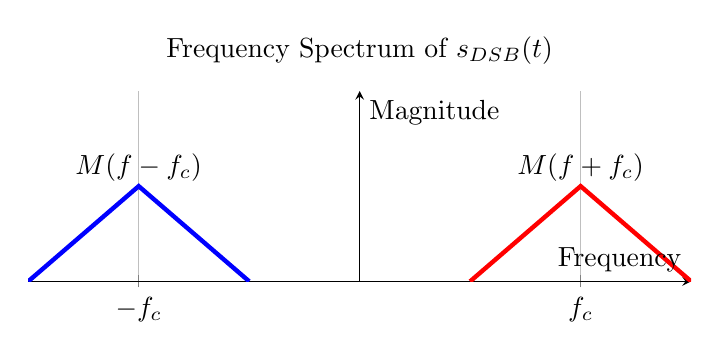
\begin{tikzpicture}
    \begin{axis}[
        title={Frequency Spectrum of $s_{DSB}(t)$},
        xlabel={Frequency},
        ylabel={Magnitude},
        xtick={-2,-1,0,1,2},
        ytick=\empty,
        ymin=0,
        ymax=2,
        grid=major,
        axis lines=middle,
        width=10cm,
        height=4cm,
        xticklabels={$-f_m$,$-f_c$,$0$,$f_c$,$f_m$},
        no markers,
        every axis plot/.append style={ultra thick}
    ]
    
    % Lower sideband
    \addplot+[sharp plot] coordinates {(-1.5,0) (-1,1) (-0.5,0)};
    \node at (axis cs:-1,1.2) {$M(f-f_c)$};
    
    % Upper sideband
    \addplot+[sharp plot] coordinates {(0.5,0) (1,1) (1.5,0)};
    \node at (axis cs:1,1.2) {$M(f+f_c)$};
    \end{axis}
\end{tikzpicture}

The DSB signal \( s_{DSB}(t) \) after being filtered by the bandpass filter (BPF) retains its form. The coherent detection is implemented by multiplying \( s_{DSB}(t) \) with a synchronized carrier \( 2\cos(2\pi f_c t) \). This results in a signal that contains the original message signal \( m(t) \) and a high-frequency component at \( 2f_c \). The low-pass filter (LPF) then removes the high-frequency component, leaving only the message signal \( m(t) \).
Using Fourier analysis, the multiplication in the time domain corresponds to a convolution in the frequency domain. Therefore, the message signal spectrum \( M(f) \) is convolved with a delta function at \( f_c \) due to the coherent carrier signal. The BPF ensures that only frequencies near the carrier frequency are passed through. After demodulation and filtering, the spectrum is centered back to baseband, recovering the message signal.
La duplicazione dello spettro giustifica il termine con cui si definisce la modulazione DSB.
Possiamo definire $B = f_c + W$ come la banda di trasmissione se consideriamo il massimo o $B = 2W$ se consideriamo quanto occupa.
Nella radio AM si ha una carrier frequency tra i 500 e i 1600 kHz e una $W$ tra i 5 e i 10 kHz.
Il segnale è pari (in modulo) a causa della simmetria hermitiana, infatti essendo $m(t)$ reale, $M(-f) = M^*(f)$ e quindi $|M(-f)| = |M(f)|$.

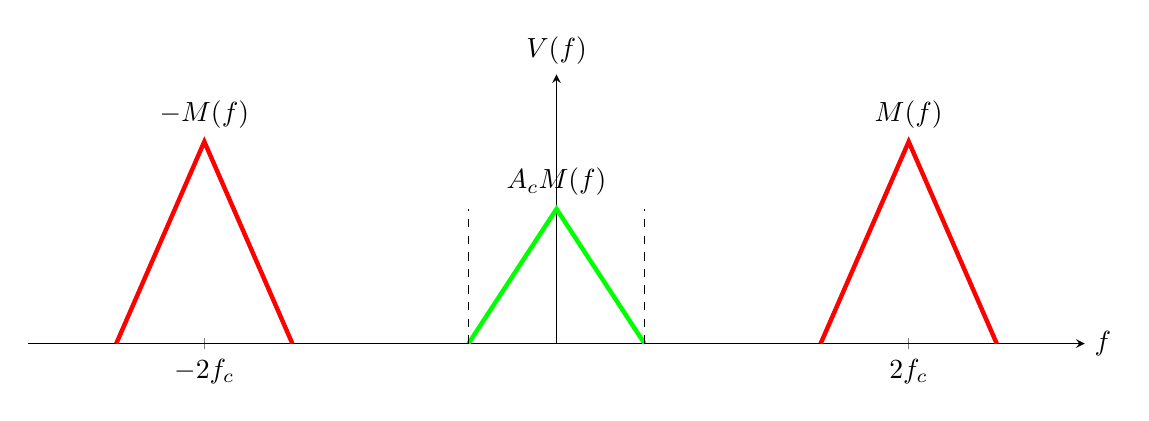
\begin{tikzpicture}
    \begin{axis}[
        width=15cm,
        height=5cm,
        axis lines=center,
        xlabel={$f$},
        ylabel={$V(f)$},
        xlabel style={at=(current axis.right of origin), anchor=west},
        ylabel style={at=(current axis.above origin), anchor=south},
        xtick={-2,0,2},
        xticklabels={$-2f_c$, $0$, $2f_c$},
        ytick=\empty,
        ymin=0,
        ymax=2,
        xmin=-3,
        xmax=3,
        no markers,
        every axis plot/.append style={ultra thick}
    ]
    % Draw the triangle peaks
    \addplot+[sharp plot, red] coordinates {(-2.5,0) (-2,1.5) (-1.5,0)};
    \addplot+[sharp plot, red] coordinates {(1.5,0) (2,1.5) (2.5,0)};

    % Draw the message signal spectrum
    \addplot+[sharp plot, green] coordinates {(-0.5,0) (0,1) (0.5,0)};
    
    % Annotations
    \node at (axis cs:-2,1.7) {$-M(f)$};
    \node at (axis cs:0,1.2) {$A_cM(f)$};
    \node at (axis cs:2,1.7) {$M(f)$};
    
    % Draw the bandwidth lines and label them
    \draw[dashed] (axis cs:-0.5,0) -- (axis cs:-0.5,1);
    \draw[dashed] (axis cs:0.5,0) -- (axis cs:0.5,1);
    \node at (axis cs:0.5,-0.2) {$W$};
    \node at (axis cs:-0.5,-0.2) {$-W$};
    \end{axis}
\end{tikzpicture}


La ricostruzione del segnale originario richiede tre step:
\begin{itemize}
  \item Filtraggio passa-banda: il segnale ricevuto è filtrato tramite un filtro passa-anda, centrato in \( f_c \), per rimuovere le componenti fuori banda.
  \item Demodulazione: il segnale modulato viene moltiplicato per un secondo coseno, ottenendo oltre al segnale originario anche due contributi in \(\pm 2f_c \)
  \item Filtraggio passa-basso: il segnale demodulato viene filtrato con un filtro passa basso di ampiezza W, per rimuovere la componente ad alta frequenza.
\end{itemize}

\begin{equation}
    v(t) = s_{DSB}(t) \cdot 2\cos(2\pi f_c t) = A_c m(t) \cdot 2\cos^2(2\pi f_c t) = A_c m(t) + A_c m(t) \cos(4\pi f_c t)
\end{equation}

L'ipotesi $f_c^{(t)} = f_c^{(r)}$ garantisce la possibilità di effettuare il passaggio trigonometrico e dunque riscostruire il segnale originario senza alcuna distorsione. Tuttavia a prescindere dalla bontà dell'oscillatore utilizzato non è possibile ottenere una sincronizzazione perfetta senza alcuna logica aggiuntiva, un reale sistema di modulazione AM prevede tale meccanismo.

\section*{Analog Quadrature Amplitude Modulation}

Per raddoppiare la quantità di informazioni trasmesse all'interno della stessa banda si può sfruttare l'ortogonalità della funzione seno e coseno, in modo da trasmettere contemporaneamente due segnali, occupando in modo ottimale la banda a disposizione. Tale modulazione è detta QAM, il termine quadrature indica lo shift di $\pi/2$ tra le due funzioni portant (seno e coseno), mentre amplitude ricorda che si tratta comunique di una modulazione in cui l'informazione è trasportata interamente dall'ampiezza del segnale. L'ampiezza del segnale portante è infatti modulata in modo proporzionale all'ampiezza del segnale modulante, contente l'informazione da trasmettere.





The composite QAM signal \( s(t) \) can be represented as the sum of two DSB-modulated signals, one modulated with a cosine (the in-phase component) and the other with a sine (the quadrature-phase component):
\begin{equation}
s_{QAM}(t) = A_{c} m_1(t) \cos(2\pi f_c t) - A_{c} m_2(t) \sin(2\pi f_c t)
\end{equation}

Where:
\begin{itemize}
    \item \( m_1(t) \) and \( m_2(t) \) are the message signals for the in-phase and quadrature-phase components, respectively.
    \item \( f_c \) is the carrier frequency.
\end{itemize}


The demodulation of the QAM signal is performed by multiplying the composite signal \( s(t) \) with \( 2\cos(2\pi f_c t) \) and \( -2\sin(2\pi f_c t) \) to retrieve the in-phase \( s_I(t) \) and quadrature-phase \( s_Q(t) \) components, respectively. These products are then passed through low-pass filters to extract the original message signals \( m_1(t) \) and \( m_2(t) \).

La demodulazione è fatta nella seguente maniera:
\begin{equation}
    v_I(t) = s(t) \cdot 2\cos(2\pi f_c t) = A_{c} m_1(t) + A_{c} m_1(t) \cos(4\pi f_c t) - A_{c} m_2(t) \sin(4\pi f_c t)
\end{equation}
\begin{equation}
    v_Q(t) = s(t) \cdot -2\sin(2\pi f_c t) = A_{c} m_2(t) - A_{c} m_1(t) \cos(4\pi f_c t) - A_{c} m_2(t) \sin(4\pi f_c t)
\end{equation}

Le componenti ad alta frequenza sono filtrate dal filtro passa-basso, ottenendo così i segnali originali \( m_1(t) \) e \( m_2(t) \).
Lo spettro del segnale ottenuto tramite moduazione non risulta più simmetrico rispetto a $f_c$, tuttavia essendo un segnale reale resta valida la simmetria rispetto all'asse delle ordinate.
La mancanza di simmetria rispetto a $f_c$ implica la non esistenza di un segnale reale in grado di rappresentare lo spettro in banda base, in quanto verrebbe meno la simmetria rispetto alla frequenza 0.
Sebbene questa mancanza non precluda l'utilizzo della modulazione QAM, nella pratica risulta più semplice lo studio di un segnale in banda base.
\begin{itemize}
    \item La carrier frequency \( f_c \) non aggiunge informazione al segnale, ma viene utilizzata per traslare il segnale in frequenza.
    \item Il criterio di Nyquist richiede un comportamente ad una frequnza doppia rispetto alla banda del segnale, quindi nel caso di segnale passa-banda tale valore può essere molto elevato. Nel caso di segnale in banda base la frquenza di campionamente può essere nettamente inferiore.
\end{itemize}

Il criterio di Nyquist stabilisce che \( T \leq \frac{1}{2B} \), dove \( T \) è il periodo di campionamento e \( B \) è la banda del segnale, e quindi \( f_s \geq 2B \). Quindi nel nostro caso, $f_s \geq 2(f_c + W)$.
Un segnale è definito in passa banda quando la propria energia è concentrata all'interno di una banda $2W$ centrata attorno a una carrier frequency $f_c$, con il vincolo $f_c >> W$.  


\subsection*{Baseband and Passband Signal Spectra}
In passband systems, a message signal with a certain bandwidth \( B \) Hz is modulated onto a carrier signal with a frequency of \( f_c \) Hz. The baseband signal spectrum represents the frequency content of the message signal, and it is usually centered at zero frequency. When the signal is modulated onto the carrier frequency, the spectrum shifts to be centered around \( f_c \), creating a passband signal spectrum.

The equation for the modulated passband signal can be expressed as:
\begin{equation}
s(t) = A_{c1} m_1(t) \cos(2\pi f_c t) - A_{c2} m_2(t) \sin(2\pi f_c t)
\end{equation}
where \( m_1(t) \) and \( m_2(t) \) represent the in-phase and quadrature components of the message signal, and \( A_{c1} \), \( A_{c2} \) are the amplitudes of the carrier.

The process of demodulation involves retrieving the original baseband signal from the modulated passband signal. The demodulated signal \( v(t) \) can be approximated by the original message signal when the carrier frequency is significantly higher than the bandwidth of the message signal, which allows for the use of simple demodulation techniques.




The received signal can be represented by the equation:
\begin{equation}
    v(t) = s(t) \cdot \cos(2\pi f_c t) + n(t)
\end{equation}

Where \( s(t) \) is the transmitted signal and \( n(t) \) is the noise.

The transmitted signal \( s(t) \) is a modulated signal with the form:
\begin{equation}
    s(t) = A_{c1} m_1(t) \cos(2\pi f_c t) - A_{c2} m_2(t) \sin(2\pi f_c t)
\end{equation}

The terms in this equation are defined as follows:
\begin{itemize}
    \item \( A_{c1} \) and \( A_{c2} \) are the amplitudes of the carrier.
    \item \( m_1(t) \) and \( m_2(t) \) are the baseband signals that modulate the carrier.
    \item \( f_c \) is the carrier frequency.
\end{itemize}

The term \( v(t) \) can also be expanded and approximated, assuming that \( m_1(t) \) and \( m_2(t) \) are limited to a bandwidth \( B \), and the carrier frequency \( f_c \) is much greater than \( B \). This approximation leads to:
\begin{align}
    v(t) & = \frac{A_{c1}}{2} m_1(t) + \frac{A_{c1}}{2} m_1(t) \cos(4\pi f_c t) + \frac{A_{c2}}{2} m_2(t) \sin(4\pi f_c t) + n(t) \\
    & = \frac{A_{c1}}{2} m_1(t) + \underbrace{A_{c1} m_1(t) \cos(4\pi f_c t)}_{\text{High frequency terms}} + \underbrace{A_{c2} m_2(t) \sin(4\pi f_c t)}_{\text{High frequency terms}} + n(t)
\end{align}

The high frequency terms can be removed using a low-pass filter, which leaves the term \( \frac{A_{c1}}{2} m_1(t) \) and the noise \( n(t) \). This is the essence of coherent demodulation, where the original message signal is recovered from the received signal.


\section*{Inviluppo Complesso di un Segnale in Banda Passante}

La maggior parte dei sistemi di comunicazione opera in banda passante. Il segnale trasmesso \( s(t) \), concentrato in una banda di frequenza \( 2B \) e centrato attorno a una frequenza portante \( f_c \), risiede ben al di sopra della corrente continua (DC) o frequenza zero. Per un segnale in banda passante, vale la condizione \( f_c \gg 2B \), indicando che la frequenza portante è molto maggiore del doppio della larghezza di banda del segnale.

L'assenza di un segnale in banda base ha portato all'adozione dell'inviluppo complesso, definito come:
\begin{equation}
    \tilde{s}(t) = s_I(t) + js_Q(t) = A(t)e^{j\phi(t)}
\end{equation}
\begin{equation}
    s(t) = \Re\{\tilde{s}(t)e^{j2\pi f_c t}\} = s_I(t)\cos(2\pi f_c t) - s_Q(t)\sin(2\pi f_c t)
\end{equation}

Questo inviluppo complesso permette di rappresentare \( s(t) \) come la parte reale del prodotto del suo inviluppo complesso per un esponenziale complesso alla frequenza portante, facilitando l'analisi e la modulazione del segnale nei sistemi di comunicazione digitale. Per esempio, nella modulazione AM si ottiene:
\begin{equation}
    \tilde{s}_{AM}(t) = m(t) = A(t)e^{j\phi(t)}
\end{equation}
dove \( \phi(t) \) assume valore \( 0 \) o \( \pi \), essendo assente la componente immaginaria.

La sincronizzazione del clock tra trasmettitore e ricevitore è cruciale per una ricostruzione perfetta dell'informazione trasmessa, mantenendo la caratteristica di ortogonalità perfetta tra seno e coseno, necessaria per separare i due messaggi una volta modulati.

L'inviluppo complesso rappresenta un modello equivalente in banda base che facilita l'analisi e l'elaborazione dei segnali in banda passante come se fossero segnali in banda base, offrendo numerosi vantaggi:
\begin{itemize}
    \item Il modello in banda base è più semplice da studiare, poiché elimina gli effetti della frequenza portante dal modello del segnale, semplificando l'analisi matematica e la comprensione delle proprietà del segnale.
    \item La simulazione numerica di un modello in banda base richiede meno risorse computazionali rispetto a un modello in banda passante, grazie alla minor larghezza di banda necessaria, riducendo quindi i costi computazionali.
    \item Di conseguenza, anche la frequenza di campionamento è inferiore per i modelli in banda base, il che si traduce in tassi di trasmissione dati ridotti, vantaggioso per l'elaborazione e lo stoccaggio del segnale digitale.
    \item Il modello in banda base è spesso la base per un'implementazione digitale di un sistema di comunicazione in banda passante, facilitando l'applicazione delle tecniche di elaborazione del segnale digitale, fondamentali nelle comunicazioni moderne.
\end{itemize}

\section*{Comunicazioni Analogiche: Modulazione di Frequenza (FM)}

Nella modulazione di frequenza (FM), il messaggio è incorporato nella fase del segnale \( \phi(t) \). Il segnale FM \( S_{FM}(t) \) può essere espresso come:
\begin{equation}
    S_{FM}(t) = A_c \cos\left(2\pi f_c t + 2\pi k_f \int_{-\infty}^{t} m(\tau) d\tau \right)
\end{equation}

La fase \( \phi(t) \) del segnale FM è quindi data dall'integrale del segnale del messaggio \( m(t) \), scalato dalla sensibilità alla deviazione di frequenza \( k_f \):
\begin{equation}
    \phi(t) = 2\pi f_c t + 2\pi k_f \int_{-\infty}^{t} m(\tau) d\tau
\end{equation}

L'indice di modulazione \( m_f \) è definito come il rapporto tra la deviazione di frequenza e la larghezza di banda del messaggio \( B_m \):
\begin{equation}
    m_f = \frac{\Delta f}{B_m}
\end{equation}

La rappresentazione complessa del segnale FM può essere ottenuta utilizzando la formula di Eulero:
\begin{equation}
    \tilde{s}_{FM}(t) = A_c e^{j\phi(t)}
\end{equation}

Espandendo \( \phi(t) \) otteniamo:
\begin{equation}
    \tilde{s}_{FM}(t) = A_c e^{j\left(2\pi f_c t + 2\pi k_f \int_{-\infty}^{t} m(\tau) d\tau\right)}
\end{equation}

Questa rappresentazione è particolarmente utile per l'analisi dei segnali FM nel contesto del trattamento digitale dei segnali.

I vantaggi della modulazione in frequenza includono:
\begin{itemize}
    \item Minore sensibilità ai disturbi, migliorando così la qualità del segnale ricevuto.
    \item Maggiore efficienza energetica, poiché il segnale informativo non richiede potenza aggiuntiva a quella della portante.
    \item L'ampliezza costante permette l'uso di amplificatori semplificati in fase di trasmissione, evitando la necessità di mantenere l'amplificatore nella zona lineare, come sarebbe necessario con le modulazioni di ampiezza variabile (AM).
    \item Possibilità di configurare la modulazione per ottimizzare il compromesso tra qualità della trasmissione e banda occupata.
\end{itemize}

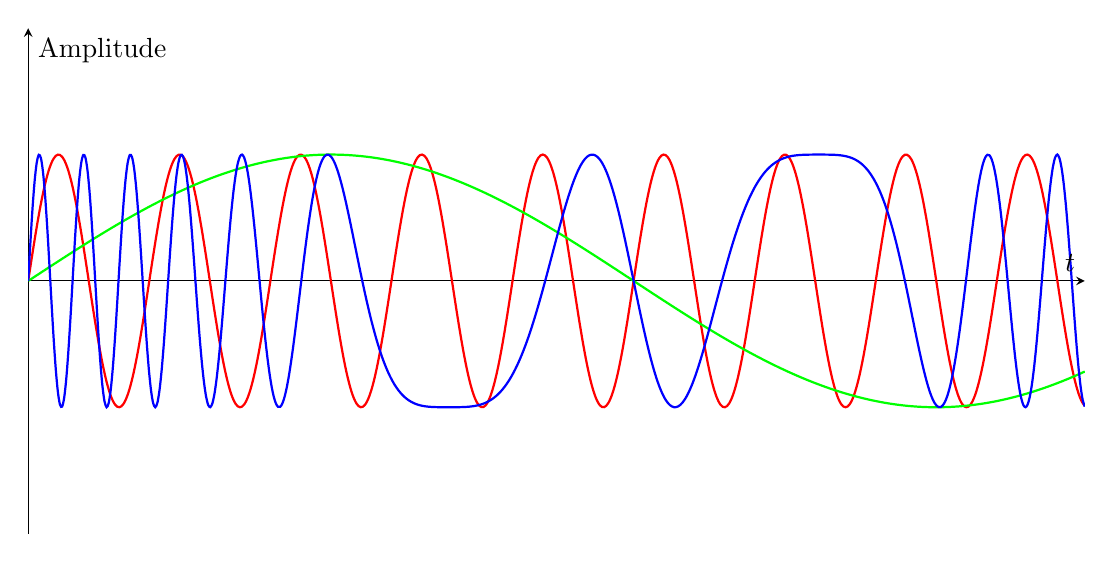
\begin{tikzpicture}
\begin{axis}[
    axis lines=middle,
    xlabel={$t$},
    ylabel={Amplitude},
    xtick=\empty,
    ytick=\empty,
    xmin=0, xmax=10,
    ymin=-2, ymax=2,
    domain=0:10,
    samples=500,
    smooth,
    width=15cm, height=8cm
]


% Carrier Signal
\addplot [red, thick] {sin(2 * pi * 50 * x)};

% Baseband Input Signal
\addplot [green, thick, domain=0:10] {sin(pi * 10*x)};

% FM Waveform (simplified representation)
\addplot [blue, thick] {sin(2 * pi * 50 * x + 1000*sin(pi * 10*x))};

\end{axis}
\end{tikzpicture}

\subsection*{FM Signal with a Modulating Sinusoid}

% Modulating sinusoid
Sia \( m(t) \) una sinusoide data da \( m(t) = V_m \cos(2\pi f_m t) \). Il segnale FM diventa:
\[
s_{FM}(t) = A_c \cos \left( 2\pi f_c t + 2\pi k_f \int_{-\infty}^{t} V_m \cos(2\pi f_m \tau) d\tau \right)
\]
che si semplifica in:
\[
s_{FM}(t) = A_c \cos \left(2\pi f_c t + m_f \sin(2\pi f_m t) \right)
\]
% Complex envelope
L'inviluppo complesso sarà:
\[
\hat{s}_{FM}(t) = A_c e^{j m_f \sin(2\pi f_m t)}
\]


Per ottenere il coefficiente di Foruier di deve risolvere l'integrale:





To compute the Fourier series coefficients for the complex envelope of the FM signal given by \( \hat{s}_{FM}(t) = A_c e^{j m_f \sin(2\pi f_m t)} \) and using your specified Fourier series integral formula, we will follow these steps:

%The integral formula to find the Fourier series coefficients \( c_n \) of the signal \( x(t) \) over one period \( T_0 \) is given by:
%\[ c_n = \frac{1}{T_0} \int_{-\frac{T_0}{2}}^{\frac{T_0}{2}} x(t) e^{-j 2\pi f_0 n t} dt \]

La formula dell'integrale per trovare i coefficienti della serie di Fourier \( c_n \) del segnale \( x(t) \) su un periodo \( T_0 \) è data da:
\[ c_n = \frac{1}{T_0} \int_{-\frac{T_0}{2}}^{\frac{T_0}{2}} x(t) e^{-j 2\pi f_0 n t} dt \]

Per la modulazione FM, dove \( f_0 = f_m \) (la frequenza di modulazione) e \( T_0 = \frac{1}{f_m} \), i coefficienti per l'inviluppo complesso \( \hat{s}_{FM}(t) \) diventano:
\[ c_n = \frac{1}{T_0} \int_{-\frac{T_0}{2}}^{\frac{T_0}{2}} A_c e^{j m_f \sin(2\pi f_m t)} e^{-j 2\pi f_m n t} dt \]

Applicando l'espansione di Jacobi-Anger, sappiamo che:
\[ e^{j z \sin \theta} = \sum_{k=-\infty}^\infty J_k(z) e^{j k \theta} \]

Quindi, con \( z = m_f \) e \( \theta = 2\pi f_m t \), otteniamo:
\[ e^{j m_f \sin(2\pi f_m t)} = \sum_{k=-\infty}^\infty J_k(m_f) e^{j k 2\pi f_m t} \]


Sostituendo l'espansione nell'integrale per \( c_n \):
\[ c_n = \frac{A_c}{T_0} \int_{-\frac{T_0}{2}}^{\frac{T_0}{2}} \sum_{k=-\infty}^\infty J_k(m_f) e^{j k 2\pi f_m t} e^{-j 2\pi f_m n t} dt \]

Scambiando la somma e l'integrale (supponendo convergenza uniforme), e notando che \( e^{j (k-n) 2\pi f_m t} \) è periodico con periodo \( T_0 \), otteniamo:
\[ c_n = \frac{A_c}{T_0} \sum_{k=-\infty}^\infty J_k(m_f) \int_{-\frac{T_0}{2}}^{\frac{T_0}{2}} e^{j (k-n) 2\pi f_m t} dt \]



L'integrale:
\[ \int_{-\frac{T_0}{2}}^{\frac{T_0}{2}} e^{j (k-n) 2\pi f_m t} dt \]
è non nullo solo quando \( k = n \), in tal caso è uguale a \( T_0 \). Altrimenti è nullo a causa dell'ortogonalità delle funzioni esponenziali su un periodo completo.


Quindi:
\[ c_n = A_c J_n(m_f) \]





La rappresentazione in serie di Fourier dello spettro dell'inviluppo complesso del segnale FM è quindi data da:
\[
\hat{S}_{FM}(t) = A_c \sum_{n=-\infty}^{\infty} J_n(m_f) e^{j 2\pi n f_m t}
\]
% FM signal spectrum representation
Il segnale FM può essere rappresentato come:
\[
s_{FM}(t) = \text{Re}\{ \hat{S}_{FM}(t) e^{j 2\pi f_c t} \} = A_c \sum_{n=-\infty}^{\infty} J_n(m_f) \cos(2\pi (f_c + n f_m) t)
\]
mostrando come la frequenza della portante sia alterata dalle frequenze del segnale di modulazione, con l'ampiezza di ciascuna componente data dai valori della funzione di Bessel.

Ogni componente sinusoidale ha una frequenza che è un multiplo intero della frequenza di modulazione \( f_m \).
Queste componenti sono chiamate "sidebands", e la loro ampiezza è determinata dalle funzioni di Bessel \( J_n(m_f) \).
La frequenza della portante appare come il picco centrale nello spettro (per \( n = 0 \)), con la sua ampiezza modulata da \( J_0(m_f) \).

In generale, l'ampiezza delle funzioni di Bessel (e quindi delle bande laterali) diminuisce all'aumentare di \( |n| \), anche se questo decadimento non è necessariamente monotono.
Il pattern esatto dipende dal valore dell'indice di modulazione \( m_f \), un indice di modulazione più alto distribuisce più energia nelle bande laterali di ordine superiore, allargando la banda del segnale FM,
infatti si può vedere graficamente come più è l'indice di modulazione, più è grande il numero di funzioni di Bessel di cui devo tenere conto quando rappresento lo spettro del segnale FM.
Lo spettro è simmetrico rispetto alla frequenza della portante perché \( J_{-n}(m_f) = (-1)^n J_n(m_f) \). Quindi, per ogni componente di frequenza positiva, c'è una corrispondente componente di frequenza negativa con la stessa ampiezza ma potenzialmente fase diversa (a seconda che \( n \) sia dispari o pari).
La banda di Carson approssima la larghezza di banda del segnale FM a:
\[
    B_{FM} \approx 2(\Delta f + f_{m}) = 2(m_f + 1) f_{m}
\]
\[
    \Delta f \coloneqq \text{max} \{ | f_d(t) | \} = k_f \cdot \text{max} \{ | m(t) | \}
\]
% TODO: qual è la differenza tra f_{max} e f_m e B?
Dove \( \Delta f \) è la deviazione massima della frequenza, \( f_{m} \) è la frequenza massima del signal modulante e \( m_f \) è l'indice di modulazione.
Questa regola stima la banda in cui è concentrata la maggior parte dell'energia del segnale FM.
Ogni segnale modulato in frequenza ha un numero infinito di bande laterali e quindi una banda infinita. Ma la maggior parte dell'energia (98\% o più) è concentrata all'interno della banda definita dalla regola di Carson. Per la radio FM mono commerciale:
\begin{align*}
f_m &= 15 \text{ kHz (high quality audio)}, \\
\Delta f &= 75 \text{ kHz}, \\
m_f &= 5, \\
B_{FM} &\approx 180 \text{ kHz}.
\end{align*}

\subsection*{FM Receiver}

% Complex envelope of the received signal
Neglecting the effect of noise and channel, the complex envelope of the received signal is
\[ \hat{v}(t) = A_c e^{j2\pi k_f \int_{-\infty}^{t} m(\tau) d\tau} \]

% Recovering the modulating signal
The modulating signal can be recovered by differentiating the phase of \( \hat{v}(t) \):
\[ \hat{m}(t) = \frac{1}{2\pi k_f} \frac{d}{dt} \Delta \hat{v}(t) \]
where \( \Delta \hat{v}(t) \) is the phase deviation of the received signal.

% Conceptual FM baseband receiver block diagram
The conceptual block diagram for an FM baseband receiver can be illustrated using a low-pass filter (L), followed by a differentiator and a demodulator to recover the message signal \( m(t) \).

% Including the block diagram in TikZ would be the next step if you want a graphical representation of the FM baseband receiver as well.
\section*{SDR (Software-Defined Radio) Concept}

% SDR concept explained
Software-defined radio (SDR) leverages modern computing power and analog-to-digital converters (ADCs) to implement radio components such as modulators, demodulators, and tuners in software, which traditionally were implemented in hardware.

\section*{SDR Paradigm}

% Details of SDR processing
In an SDR system, the incoming signal is converted to a digital format and then processed digitally. This allows for the radio hardware to be largely programmable and configurable by software, making it possible to update and adapt the system to new modulation formats, algorithms, and applications easily.

% Benefits of SDR
SDR platforms offer versatility across various products and applications, potentially reducing costs and either maintaining or enhancing performance.



\begin{tikzpicture}[
    block/.style={rectangle, draw, minimum height=2em, minimum width=3em},
    line/.style={draw, -Latex}
]


% create the node antenna with image imgs/antenna.pdf

% Define nodes
\node[block, align=center] (rfFrontEnd) {Flexible RF \\ Front End};
\node[block, right=0.5cm of rfFrontEnd, align=center] (adConverter) {A/D Converter};
\node[block, right=0.5cm of adConverter, align=center] (demod) {Demodulation \\ to Bband};
\node[block, right=0.5cm of demod, align=center] (decimation) {Decimation \\ Filtering};
\node[block, right=0.5cm of decimation, align=center] (carrierSync) {Carrier \& Timing \\ Synchronisation};
\node[block, right=0.5cm of carrierSync, align=center] (baseband) {Baseband \\ Processing};
% before rfFrontEnd, and upper of it of 0.5cm
\node[inner sep=0pt, outer sep=0pt, above left=0.25cm and 0.05cm of rfFrontEnd] (antenna) {
\includegraphics[width=1cm]{imgs/antenna.pdf}};

% Connect blocks with arrows
\draw[line] (rfFrontEnd) -- (adConverter);
\draw[line] (adConverter) -- (demod);
\draw[line] (demod) -- (decimation);
\draw[line] (decimation) -- (carrierSync);
\draw[line] (carrierSync) -- (baseband);
% Draw antennae
\draw (rfFrontEnd.west) -- ++(-0.5, 0) -- ++(0,0.5);


% Group hardware and software parts
\node[draw, dashed, fit=(rfFrontEnd) (adConverter) (demod) (decimation), inner sep=0.2cm, label=above:RTL-SDR Hardware] (hardware) {};
\node[draw, dashed, fit=(carrierSync) (baseband), inner sep=0.2cm, label=above:MATLAB / Simulink design (running on computer)] (software) {};

% Add frequency range and sampling frequency annotations
\node[align=left, below=0.5cm of hardware.south] (freqRange) {Range: \\ 25MHz -- 1.75GHz};
\node[align=left, below=0.5cm of software.south] (samplingFreq) {Sampling frequency (\(f_s\)): \\ up to around 2.8MHz};

% Baseband output symbol
%\node[right=0.5cm of baseband] (output) {\(\musicalnote\)};
% create a node with a background image imgs/notes.svg
\node[inner sep=0pt, outer sep=0pt, right=0.5cm of baseband] (output) {
\includegraphics[width=1cm]{imgs/notes.pdf}};
\draw[line] (baseband) -- (output);
\end{tikzpicture}
\











\section*{SDR – Historical Milestones}

% Timeline of SDR development
Notable historical milestones in the development of SDR include:
\begin{itemize}
    \item \textbf{1984:} E-Systems Inc. (Raytheon) coined the term 'software radio.'
    \item \textbf{1991:} SPEAKeasy, the first military radio program specifically requiring software radios, is initiated.
    \item \textbf{1992:} J. Mitola publishes a paper on 'Software Radios: Survey, Critical Analysis and Future Directions.'
    \item \textbf{2005:} Ettus Research introduces the USRP, the first commercial SDR, setting a standard for open-source, hardware GNU radio.
    \item \textbf{2011:} A Finnish hacker discovers that the Realtek RTL2832U chip could be forced to operate in test mode, outputting raw I/Q data, marking a significant point in SDR accessibility.
\end{itemize}


\section*{Programmable Hardware for SDR}

% Types of programmable hardware used in SDR
There are various types of programmable hardware that facilitate the development of SDR:
\begin{enumerate}
    \item \textbf{Reconfigurable Radio:} Typically FPGA-based, these devices offer a high degree of flexibility and are often used for prototyping and research.
    \item \textbf{Programmable Radio:} Devices like DSPs or hybrids of FPGA/DSP are used for more specific applications where dedicated processing is required.
    \item \textbf{Fully Software Radio:} Utilizes General-Purpose Processors (GPP) like the Intel Core i7 for all radio functions, leveraging the processing power of modern CPUs.
\end{enumerate}

\section*{Telecom Services in the 0.1-2.5 GHz Band}

% Telecom frequency bands
The frequency spectrum from 0.1 to 2.5 GHz is populated with various telecom services, each occupying a specific band:
\begin{itemize}
    \item \textbf{AM Radio} is found in the lower frequencies, typically below 1 MHz.
    \item \textbf{FM Radio and TV Broadcasts} generally occupy the spectrum from 88 to 108 MHz and 470 to 862 MHz, respectively.
    \item \textbf{Mobile Services} such as 2G, 3G, and 4G span across multiple bands, from 700 MHz to over 2 GHz.
    \item \textbf{Wi-Fi} operates in bands around 2.4 GHz and 5 GHz.
    \item \textbf{Satellite Communications} and \textbf{GPS} also have designated bands within this range.
\end{itemize}
This band is essential for communication services and is carefully regulated to prevent interference between different services.

\section*{RTL-SDR Architecture}

% Detailing the components of RTL-SDR
The RTL-SDR is a popular SDR device that comprises several key components:
\begin{itemize}
    \item \textbf{R820T DTV Tuner:} Responsible for selecting the desired signal frequency band from the RF spectrum.
    \item \textbf{28.8MHz Clock Crystal:} Provides a stable reference frequency for the tuner and demodulator.
    \item \textbf{RTL2832U COFDM Demodulator:} Demodulates the digital signal from the tuner.
    \item \textbf{MCX Antenna Connector:} Allows for the connection of various types of antennas.
    \item \textbf{Serial EEPROM:} Stores the configuration data for the USB device.
    \item \textbf{USB 2.0 Interface:} Facilitates the connection with computers for further processing.
    \item Additional components such as a \textbf{Power LED}, \textbf{ESD Diode}, and \textbf{IR Sensor} for user interfacing and device protection.
\end{itemize}

\section*{SDR Block Diagram for an FM Receiver}

% Explanation of the SDR block diagram for FM reception
The block diagram for an FM receiver using RTL-SDR hardware typically involves the following processing stages:
\begin{enumerate}
    \item \textbf{RF Antenna:} Captures the FM signal from the air.
    \item \textbf{Flexible RF Front End:} Filters and amplifies the RF signal from the antenna.
    \item \textbf{Analogue to Digital Converter (ADC):} Converts the analog RF signal to a digital format.
    \item \textbf{Demodulation to IQ Band:} The digital signal is demodulated into I (In-phase) and Q (Quadrature) components.
    \item \textbf{Decimation Filtering:} Reduces the sampling rate and noise, retaining the signal of interest.
    \item \textbf{Carrier \& Timing Synchronization:} Synchronizes the received signal with the local reference for accurate demodulation.
    \item \textbf{Baseband Processing:} This may involve MATLAB/Simulink running on a computer to process the demodulated signal.
    \item \textbf{Baseband Output:} The final audio signal is output, ready for listening.
\end{enumerate}
The signal processing range for this system is from 25MHz to 1.75GHz with a sampling frequency (IF) up to around 2.8MHz.


\section*{RTL-SDR Receiving Steps}

% Detailed steps of the RTL-SDR superheterodyne receiver chain
The RTL-SDR device functions as a superheterodyne receiver, processing signals through the following steps:
\begin{enumerate}
    \item \textbf{Mixing to Intermediate Frequency:} Incoming signals are mixed down to an intermediate frequency (IF) of 3.57 MHz, which allows for easier signal processing and better selectivity and sensitivity.
    \item \textbf{Sampling by ADC:} The IF signal is then sampled by a two-channel (I/Q) 28.8 MS/s 8-bit analog-to-digital converter (ADC), turning the analog signal into a digital format.
    \item \textbf{Digital Downconversion:} The digitized I/Q data passes through parallel paths in a digital downconversion process that includes mixing, filtering, and decimating the input signal to a user-specified rate. The maximum sampling rate after decimation can reach approximately 2.8 MS/s.
    \item \textbf{Data Transfer to Host:} Finally, the downconverted samples are transferred to the host computer via a standard USB connection for further processing and analysis.
\end{enumerate}
This process outlines the steps involved in the digital reception and conversion of RF signals in the RTL-SDR system.


\section*{RTL-SDR Block Diagram}
The process of converting an RF signal to a baseband signal in an RTL-SDR involves several steps, illustrated in the block diagram and detailed equations:
\begin{enumerate}
    \item The RF signal undergoes amplification and filtering, including active gain control and rejection of RF image frequencies.
    \item The analog signal is mixed down to an intermediate frequency (IF) of 3.57 MHz to suit the ADC sampling rate.
    \item The ADC samples the IF at 28.8 MS/s and then the signal is filtered and decimated.
    \item Digital downconversion is performed using quadrature numerically-controlled oscillators (NCOs) to generate in-phase (I) and quadrature (Q) components.
    \item The digitized I/Q data is then resampled and synchronized, outputting to the USB port at a lower rate (up to 2.8 MS/s) and passed to software like MATLAB/Simulink for further processing.
\end{enumerate}
This process effectively moves the signal from the RF spectrum into the digital domain, where it can be manipulated and analyzed with much greater flexibility.

The RF signal is converted to baseband through the following mathematical steps:

\begin{enumerate}
    \item The received RF signal at frequency \( f_c \) is mixed with a local oscillator signal to shift its frequency down to the intermediate frequency (IF):
    \[ S_{IF}(t) = S_{RF}(t) \cdot \cos(2\pi f_{LO} t) \]
    where \( f_{LO} \) is the local oscillator frequency chosen such that \( f_{IF} = |f_{LO} - f_c| \).

    \item The resulting IF signal is then sampled by an ADC at a sampling frequency \( f_s \):
    \[ S_{ADC}(n) = S_{IF}(nT_s) \]
    where \( T_s = \frac{1}{f_s} \) is the sampling period, and \( n \) is the discrete sample index.

    \item The digitized signal undergoes digital downconversion (DDC), which includes mixing, filtering, and decimation to reduce the sample rate to a lower intermediate frequency:
    \[ S_{DDC}(t) = S_{ADC}(t) \cdot e^{-j2\pi f_{IF} t} \]
    followed by low-pass filtering to isolate the baseband component.

    \item The complex baseband signal \( S_{BB}(t) \) is obtained:
    \[ S_{BB}(t) = \text{LPF}\{S_{DDC}(t)\} \]
    which represents the in-phase (I) and quadrature (Q) components of the original RF signal.
\end{enumerate}
These steps translate the high-frequency RF signal into a lower frequency baseband signal that can be further processed by software applications for various communication tasks.